
\begin{figure}[h!]
    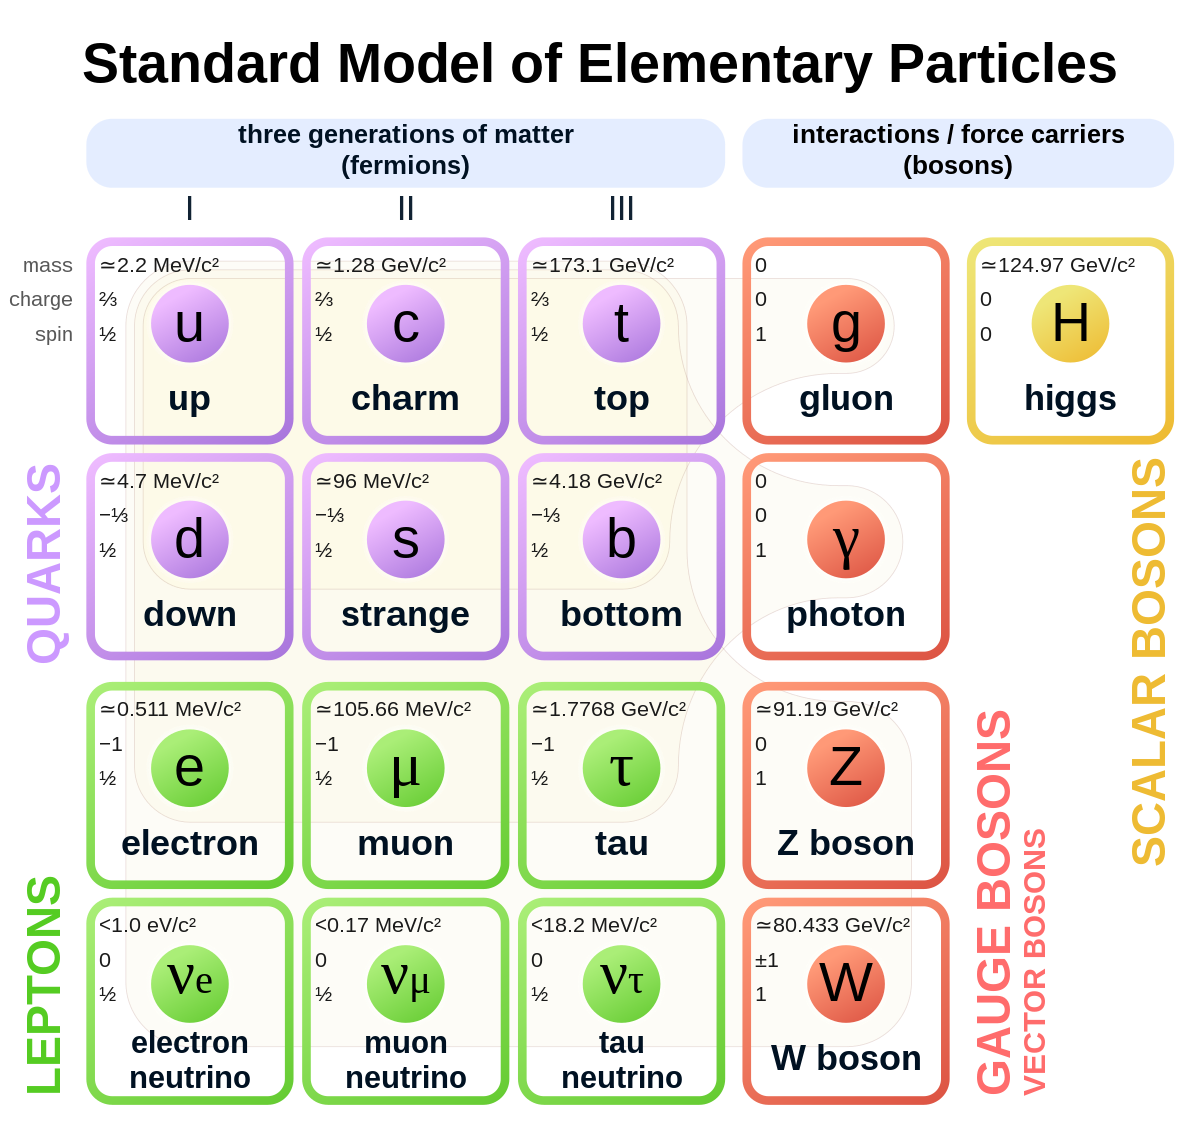
\includegraphics[width=\linewidth]{Figures/SM/Standard_Model_of_Elementary_Particles.svg.png}
    \caption{The standard model of elementary particles. Source \href{https://upload.wikimedia.org/wikipedia/commons/thumb/0/00/Standard_Model_of_Elementary_Particles.svg/1200px-Standard_Model_of_Elementary_Particles.svg.png}{here}. Accessed 07.10.22}
    \label{fig:smdiagram}
\end{figure}

\section{Structure and composition of the Standard Model}
This section will describe the standard model in a phenomelogical way, as the mathematics and physical reasoning behind the theory is not of great 
importance to understand the work, nor the results or discussion of them. For a more technical explanation, read (Pich, 2008)\cite{Pich:819632} for a 
well written paper containing the some more standard model fundamentals, as well as summarizing the experimental status regarding the standard model.
For more mathematical understanding of the standard model, Peskin and Schroeder's "An introduction to Quantum Field theory" (Peskin and Schroeder, 1995)\cite{Peskin:1995ev}
 is highly recommended. Finally, for more understanding of particle physics, the nature of interactions and more, see Thomson's "Modern Particle physics" (Thomson, 2013)\cite{Thomson:2013zua}. \par


The standard model is to physicists what the periodic table is to chemists. It is comprised of two parent class particles, fermions and bosons, where fermions 
are comprised of quarks and leptons. The model contains 17 particles, 6 quarks, 6 leptons and 5 bosons, and are shown in figure \ref{fig:smdiagram}.



\subsection*{Fermions}
The fermions are the building blocks of matter, and contain two types of particles, leptons and quarks. Together they form protons and neutrons,  atoms all around us.
Fermions, unlike bosons, are spin half particles, and are also the only particles to have anti particles. The fermions are grouped into three so called families:
\begin{equation*}
    \begin{bmatrix}
        \nu_e & u \\
        e^{-} & d^{\, '} 
    \end{bmatrix},\quad
    \begin{bmatrix}
        \nu_{\mu} & c \\
        \mu^{-} & s^{\, '}
    \end{bmatrix},\quad
    \begin{bmatrix}
        \nu_{\tau} & t \\
        \tau^{-} & b^{\, '}
    \end{bmatrix}
\end{equation*}
Note that the left column contains the leptons. whilst the right column contains the quarks. Within the left column, the subscripted $\nu$ denotes what kind of neutrino that corresponds 
to the given lepton. Here, the first family consists of the electron, the electron neutrino, the up and down quarks. The second family consists of the muon and the
muon neutrino, the charm and strange quarks. The third family consists of the tau and the tau neutrino, the top and bottom quarks. The masses of these particles 
increases for each particle in the matrix as the family number increases, i.e the muon is heavier than the electron, and the tau is heavier than the muon, and so 
on for the other fermions. \par
Quarks are fractional charge particles, with defined charge of either $2/3$ or $-1/3$. They are the "main" building blocks of protons and neutrons, and are bound by the strong 
force, the strongest of the four fundamental forces. The force mediator is the gluon. The other half of fermions are the leptons. They are split into the charged 
leptons (electrons, muons and taus), and the uncharged leptons (neutrinos). The charged leptons can interact via the electroweak force, where the Z, W bosons 
as well as the photon can be a mediator.


\subsection*{Bosons}
Bosons are integer number spin particles, with spin $0, 1, 2, ...$. Within bosons there are so called elementary bosons, some of which are force carriers or mediators such as the W, Z and the photon.
The Higgs boson is also an elementary boson, but is not a force carrier. It provides masses for the fermions via spontaneous symmetry breaking\cite{Pich:819632}. Other 
bosons are so called composite bosons, which are particles constructed by an even amount of fermions yeilding the integer spin. 

\subsection*{Left and right handedness}
Particles in the standard model are subject to a quantum mechanical property called chirality. 
Chirality is a property that describes a particle's ability to be superimposed on its mirror image. 
If a particle has chirality, it cannot be superimposed on its mirror image by any combination of translation, 
rotation, and reflection operations. \cite{weinberg_1995}

\subsection*{Feynman diagrams}
A graphical way to understand particle interactions are through so called Feynman diagrams. Feynman diagrams are drawn based on the Feynman rules for a given Lagrangian\cite{Pich:819632}\cite{feynrules}, and each component 
can be linked to a part in the Lagrangian for the system. 

\begin{figure}[h!]
    \centering
    \caption{Feynman diagram of muon pair production from electron scattering. Here, both Z and $\gamma$ can work as the propagator.}
    
\begin{tikzpicture}
    \begin{feynman}
    
        \vertex at (0.5, 1.) (a2){\(e^{-}\)} ;
        \vertex at (0.5, -1.)  (a5){\(e^{+}\)} ;

        \vertex at (1.5, 0.0) (c);
        \vertex at (3., 0.0) (d);

        \vertex at (4, 1.) (f1) {\(\mu^{-}\)} ;
        \vertex at (4,-1.) (f2) {\(\mu^{+}\)};

        
    \diagram*{


        (a2) -- [fermion] (c) -- [boson] (d),
    
        (a5) -- [anti fermion] (c) -- [boson, edge label = {$\gamma, Z$}] (d),
        (d) -- [fermion] (f1),
        (d) -- [anti fermion] (f2),
        
        ;
    };
    \end{feynman}
    \end{tikzpicture}
    \label{fig:eemm_scat}
\end{figure}

In figure \ref{fig:eemm_scat} we have a Feynman diagram describing two scenarios: electron scattering into muon pairs and 
electron muon scattering into electron muon. This is because we have not yet set the direction for time evolution. In this thesis, all 
diagrams will be interpreted from left to right, i.e figure \ref{fig:eemm_scat} then only represents electron scattering into muon pair. 
The diagram contains all the components in the Lagrangian, and arrows, curly lines and so on all have its own meaning. A straight line with 
an arrow usually means a fermion, where the direction of the arrow tells if the particle (arrow towards the vertex) is an anti particle (arrow away from the vertex) 
or particle, showing the momentum direction essentially. The is often also a propagator between the input and the output of such processes, 
and they depend on the processes we want to study. in the diagram above we have lepton scattering, thus we can both have the photon and the 
Z-boson as a propagator. This process is called a neutral current\cite{Pich:819632}, as the total charge coming out of the interaction is 0. 
As with neutral currents, we also have so called charged currents, where the sum of charge is not 0. Note that we only require charge conservation,
thus there is nothing wrong with either having a neutral or a charged current, as long as charge conservation is preserved. \par 
Feynman diagrams is not only used for visualizing scatterings, they can also visualize decays. An example is provided below. 

\begin{figure}[h!]
    \centering
    \caption{Muon decay into an electron, an electron neutrino and a muon neutrino via the $W^{-}$ boson. Read the graph from left to right.}
    
\begin{tikzpicture}
    \begin{feynman}
    
        \vertex at (0.5, 0.) (a2){\(\mu^{-}\)} ;

        \vertex at (2., 0.0) (c);
        \vertex at (3., -1.) (d);
        
        \vertex at (3.5, 0.7) (a3){\(\nu_{\mu}\)} ;

        \vertex at (4, -0.5) (f1){\(e^{-}\)} ;
        \vertex at (4.,-1.4) (f2) {\(\bar{\nu}_{e}\)};

        
    \diagram*{


        (a2) -- [fermion] (c) -- [boson, edge label = {$W^{-}$}] (d),
        (a2) -- [fermion] (c) -- [fermion] (a3),
        (d) -- [fermion] (f1),
        (d) -- [anti fermion] (f2),
        
        ;
    };
    \end{feynman}
    \end{tikzpicture}
    \label{fig:eemm_scat}
\end{figure}

Here we have a decay of a muon into and electron and two neutrinos, through a charged current. 

\subsection*{Some limitations}
All though the standard model have had great success comparing with experiments,
there are still several problems not addressed by it. One example is gravity, the standard model
as described above, does not and cannot explain gravity in a quantized way. There 
are models that try to address this problem, but they supplement the standard model,
and does not derrive it from it. \par 
The problem that will be addressed in this thesis is a curious property of the weak interaction, 
namely that parity is broken. Parity as a mathematical operation is equivalent to the spatial inversion 
through the origin\cite{Thomson:2013zua}:
\begin{equation}
    x \to -x.
\end{equation}
In other words, parity can be thought of as left-right symmetry, or mirror symmetry. Breaking of parity is observed
with weak currents, where the mediator of the charged currents, $W^{\pm}$ only interacts with 
left handed fermions. In the standard model, neutrinos are assumed to be massless, and the righthanded 
neutrinos are sterile, i.e they do not interact with the standard model. \par 
This asymmetry is strange, and hints towards new physics that perhaps can restore the parity breaking. 
Another note to make is that it has been experimentally verified that the neutrinos are massive\cite{Katrin_neutrinos},
with an upper limit on the mass for the anti electron neutrino of $m_{\nu} < 0.8eVc^2$ at $90\%$ confidence level.
This is somewhat problematic, as the masses of the neutrinos are not predicted by the standard model. 








